\chapter{Графен}
Для ознакомления с перечисленными выше пакетами в качестве примера использовался лист графена. Выбор обусловлен тем, что с одной стороны это основа сверхрешёток, которые будут изучаться в дальнейшем, а с другой стороны в литературе представлена зонная структура графена и полученные в ходе работы программы результаты есть с чем сравнивать.

\begin{figure}[h]
    \center
    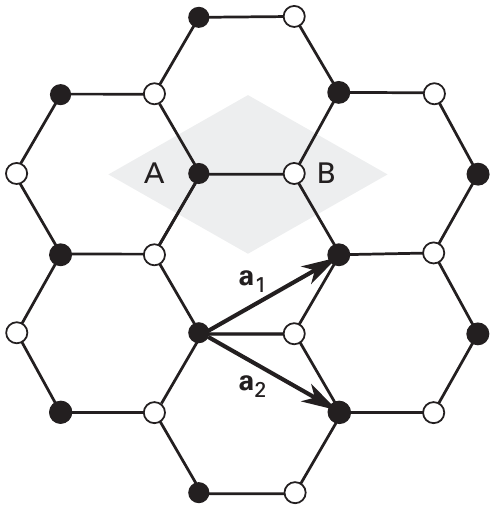
\includegraphics[width=.4\textwidth]{gra}\hfill
    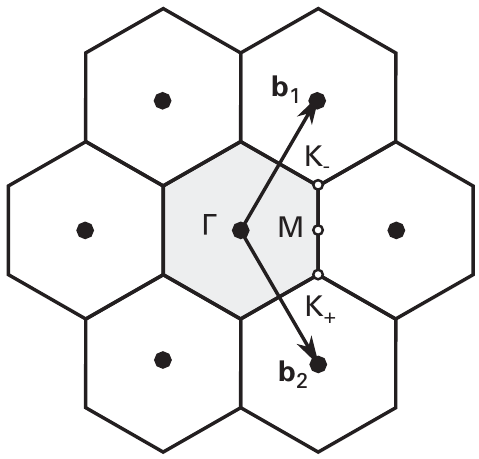
\includegraphics[width=.4\textwidth]{grb}
    \parbox[t]{.4\textwidth}{\center а)}\hfill
    \parbox[t]{.4\textwidth}{\center б)}
    \caption{Прямая (а) и обратная (б) решётки графена}
    \label{graphene}
\end{figure}

Графен представляет из себя двухмерный кристалл, в узлах кристаллической решётки которого располагаются атомы углерода. Он обладает гексагональной решёткой, в элементарной ячейке которой находятся 2 атома (рисунок~\ref{graphene}а). Обратная решётка также гексагональна, поэтому зона Бриллюэна имеет форму шестиугольника (рисунок~\ref{graphene}б).

Характерной особенностью зонной структуры графена является так называемый конус Дирака. В углах шестиугольной зоны Бриллюэна (в точках K) зона проводимости пересекается с валентной зоной, причём закон дисперсии вблизи этих точек линеен. Поэтому вблизи них поверхность \(E(\vec{k})\) представляет собой конус. Вершина этого конуса располагается на уровне Ферми.